\documentclass[12pt]{report}
\usepackage{graphicx}
\usepackage{listings}
\usepackage{cite}

% Document setup
\graphicspath{ {img/} }
\title{CSCI-476 Final Test}
\date{May 6, 2015}
\author{Gunnar Holwerda}
\renewcommand*\contentsname{Table of Contents}
\newcommand{\mychapter}[2]{
    \setcounter{chapter}{#1}
    \setcounter{section}{0}
    \chapter*{#2}
    \addcontentsline{toc}{chapter}{#2}
}

% Begin actual report

\begin{document}

\begin{titlepage}

\newcommand{\HRule}{\rule{\linewidth}{0.5mm}} % Defines a new command for the horizontal lines, change thickness here

\center % Center everything on the page

\textsc{\LARGE Montana State University}\\[1.5cm] % Name of your university/college
\textsc{\Large Hint, BlackBox, RedTeam}\\[0.5cm] % Major heading such as course name
\textsc{\large mthack.me}\\[0.5cm] % Minor heading such as course title


\HRule \\[0.4cm]
{ \huge \bfseries CSCI-476 Final Practicum}\\[0.4cm] % Title of your document
\HRule \\[1.5cm]

\Large \emph{Author:}\\
Gunnar \textsc{Holwerda}\\[3cm] % Your name

{\large \today}\\[3cm] % Date, change the \today to a set date if you want to be precise

\vfill % Fill the rest of the page with whitespace

\end{titlepage}

\tableofcontents
\clearpage

\mychapter{0}{Executive Summary}
Over the course of my time exploring the MHK's domains I was able to find many exploits. In my first phase of exploration there were open ssh and telnet ports on a couple subdomains that I was able to exploit. Then on a certain subdomain I was able to download the private ssh key from the server through my web browser.\\
\newline
During phase two I was able to find a subdomain with tomcat installed and open to the public. It had default credentials which allowed me to upload a payload to the site and get a reverse shell. In phase 3 I was able to edit a binary, using radare2, to edit the assembly of a binary to get me past a password check and allowed me to find the name to a secret html file.\\
\newline
Phase 4 involved me sifting through a file system using the DFF GUI to extract sensitive data that was witheld within. Finally, in phase 5 I was able to filter the strings out of a pcap file using strings to find the last bit of sensitive data I needed to complete this report.\\
\newline
Overall I feel that the MHK have not protected their servers well from outside attack and would give them and overall ranking of 3 / 10.
\clearpage

% Begin Round 1

\mychapter{1}{Round 1}
\section{DiscoveredIn1655}

When starting out I was given the information that the members of mhk had been discussing RFC2100. This RFC mentions a few names, so I began using the names mentioned as subdomains of mthack.me and quickly found titan.mthack.me. I ran nmap on the host to see what ports were open.\\
	\begin{verbatim}
	$	nmap -sS -p1-65535 titan.mthack.me -v -T4
	\end{verbatim}
The nmap returned that port 22 and 23 were open. I attempted to ssh, but found that a public key was needed. Next I used telnet to connect to port 23 and was presented with my first flag ``DiscoveredIn1655''.\\
\newline
\begin{center}
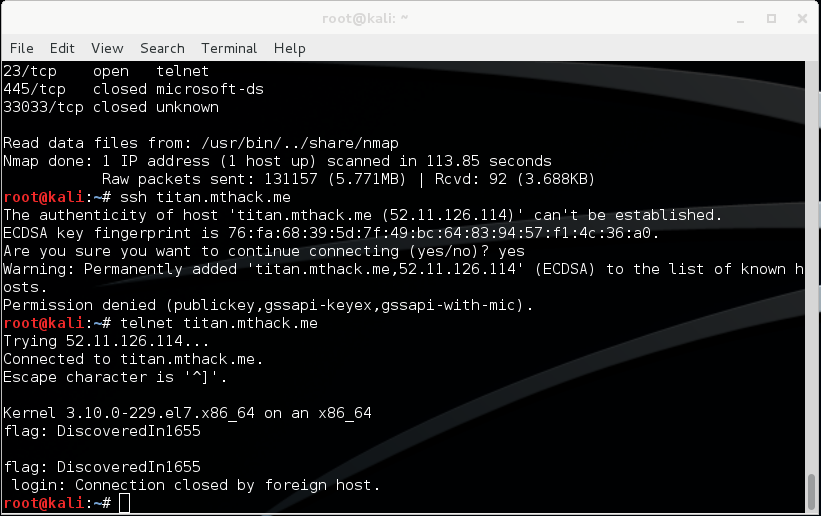
\includegraphics[scale=0.33]{DiscoveredIn1655.png}
\end{center}
\section{Th1sT1m3ItsAMoon}

In addition to titan.mthack.me, I was able to find the europa.mthack.me subdomain. After an nmap on europa I saw that port 7870 was open. There was no information about this port, so I used NetCat to connect to it, it returned ``SSH-2.0-OpenSSH\_6.6.1''. After seeing this I knew that I should use SSH to connect to europa.mthack.me on this port.
	\begin{verbatim}
	$	ssh europa.mthack.me -p 7870
	\end{verbatim}
After adding europa to my known\_hosts I was presented with my second flag ``Th1sT1m3ItsAMoon''.\\
\newline
\begin{center}
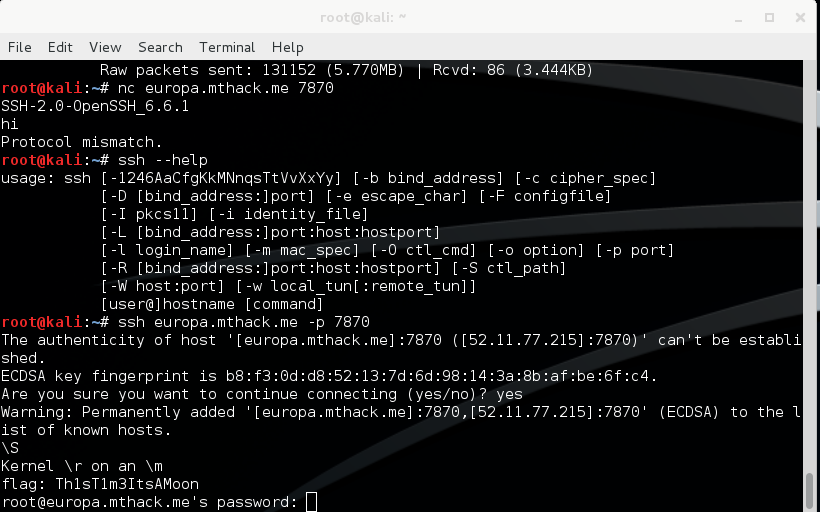
\includegraphics[scale=0.33]{Th1sT1m3ItsAMoon.png}
\end{center}
\section{SocialContract}

Another subdomain that I found during my investigation was hobbes.mthack.me. When visiting the subdomain in a browser you are presented with a webpage that says ``hi''. I decided to try to run dirbuster to see if there were any files that were accessible on the server through the browser. After many attempts with the built in directory wordlists in Kali, I downloaded a new set \cite{jrivard2009} and ran the ``Crazy'' version of the wordlist. This returned that /~root/ssh was accessible. There was a file in the directory leading me to the ``.ssh'' folder. I downloaded the private key from the server using:
	\begin{verbatim}
	$	wget hobbes.mthack.me/~root/.ssh/id_rsa
	\end{verbatim}
I then moved the key to my .ssh directory and ran:
	\begin{verbatim}
	$	ssh thomas@hobbes.mthack.me
	\end{verbatim}
There was a text file in the home directory, I opened it up, and found the final flag in Round 1 ``SocialContract''.\\
\newline
\begin{center}
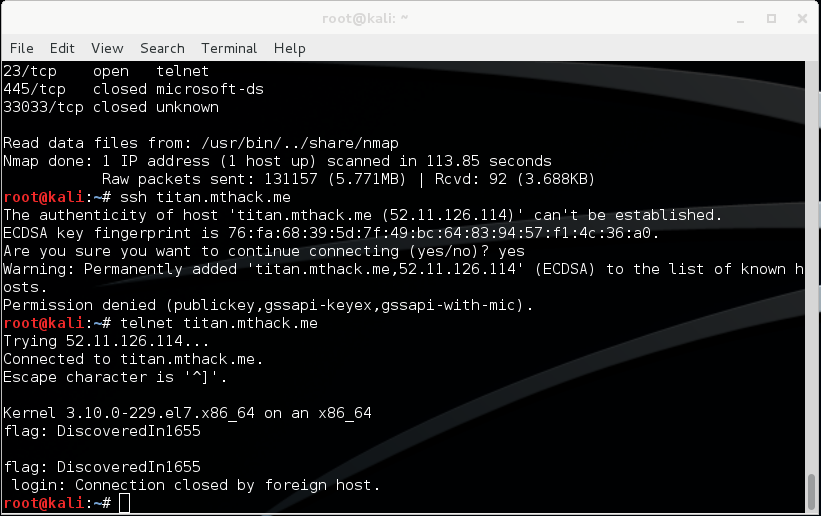
\includegraphics[scale=0.33]{DiscoveredIn1655.png}
\end{center}

% Begin Round 2

\mychapter{2}{Round 2}
\section{TomcatIsAVulnerability}

The information for Round 2 led me to mercury.mthack.me. I used nmap on the host and discovered that port 8089 was open, but was unknown. After using netcat to try to tell what the service was, I opened up mercury.mthack.me:8089 in my browser. I was then presented with the Tomcat homepage. I tried to login as the manager with ``tomcat'', ``tomcat'' as my username and password and was successful in logging in.\\
\newline
After trying multiple exploits and payloads through metasploit, I eventually found a website \cite{tonylee2012} that provided me with a payload that I could upload which gave me a shell through the browser. I uploaded that file and started navigating the filesystem looking for a file. After about 20 minutes of unsuccessul searches I decided to start listing everything ordered by time. I figured that the flag would be in a directory that had been modified most recently. This strategy led me to /opt/ where the flag.txt file was residing. I opened the file and was presented with the flag from round 2, ``TomcatIsAVulnerability''.\\
\newline
\begin{center}
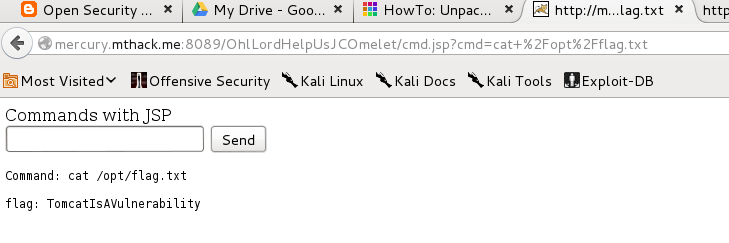
\includegraphics[scale=0.33]{TomcatIsAVulnerability.png}
\end{center}

% Begin Round 3

\mychapter{3}{Round 3}
\section{nextlevel}
Given the binary for round three, I first ran strings on the file using grep to try to find ``password'' or something along those lines. These attempts were unsuccessful, so I moved onto editing the binary using radare2. I was able to find the location of a ``jnz'' instruction right after asking for the number. I edited that instruction to be a ``jz'' instead and was presented with ``ciph3rfun.html''.\\
\newline
I then visited www.mthack.me/ciph3rfun.html and was presented with some sort of enocded flag. It looked like ROT, so I went to a ROT decoder, entered the cipher text and was presented with the flag ``nextlevel''.\\
\newline
\begin{center}
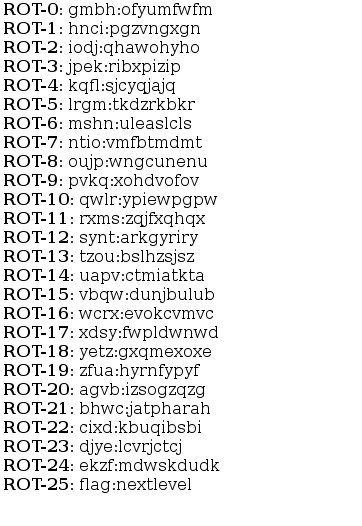
\includegraphics[scale=0.75]{nextlevel.png}
\end{center}
% Begin Round 4

\mychapter{4}{Round 4}
\section{FSInc3ption}
I downloaded mhk.exe from mthack.me/test, and ran file on it to see what sort of file it was. The output told me that it was a file system. I decided to use DFF GUI on it for my forensic tool and saw that in the file system there were two files: .mhk-warez-login-info.zip and m0ar-secrets.dd. I extracted the .dd file from mhk.exe and opened that in DFF GUI to find flag.txt. Giving me my first flag of round 4: ``FSInc3ption''.\\
\newline
\begin{center}
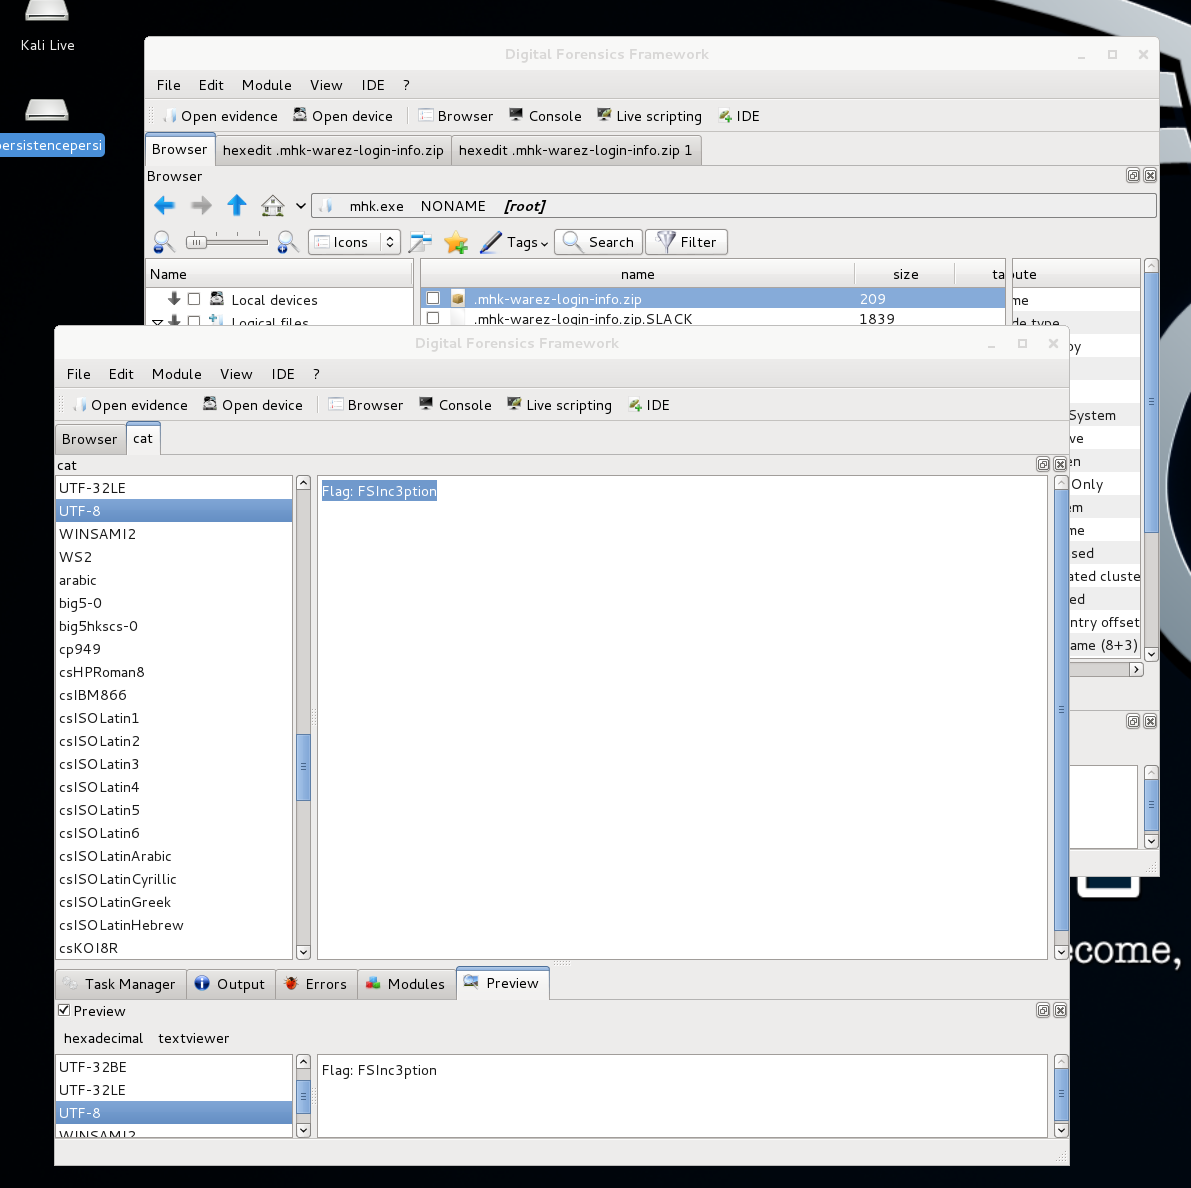
\includegraphics[scale=0.33]{FSInc3ption.png}
\end{center}

\section{deaddrop}
I switched my attention towards the .mhk-warez-login-info.zip file. When trying to unzip it, I was presented with a prompt to enter the password. I thought that the file may be encrypted using true encrypt, I ran truecrack on it but the password wasn't cracked. Eventually I found the fcrack tool which is used to brute force passworded zip files.\\
	\begin{verbatim}
	$	fcrack -v -D -p metasploit-jtr/password.lst mhk-warez-login-info.zip
	\end{verbatim}
After an hour of looking at the help text, and setting up the correct flags It was able to find the correct password of ``blessed''. After it unzipped I had the flag.txt file and opened it up to find my second flag of Round 4: ``deaddrop''.\\
\begin{center}
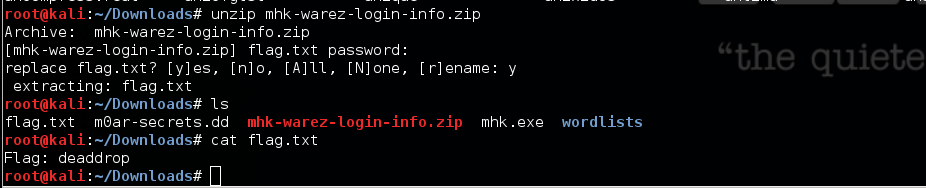
\includegraphics[scale=0.33]{deaddrop.png}
\end{center}

\mychapter{5}{Round 5}
\section{haxtheplanet}
Given the pcap for Round 5, I ran strings on the file using grep to filter out for ``flag:'', this gave me another flag: ``haxtheplanet''.\\
\newline
\begin{center}
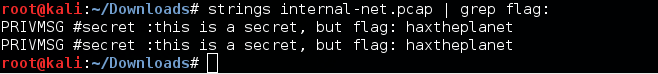
\includegraphics[scale=0.5]{haxtheplanet.png}
\end{center}

\mychapter{6}{Misc. Flags}
\section{mylittlepwnie}
On the second day of the test, the homepage for mthack.me was updated to include a username and password login form. I knew from before that the source of the webpage contained some comments so I decided to view the source of the page. I found the <script> tag linking the login form to login.js. In the javascript it was directly comparing if the login was ``root:toor''. I used those credentials to login to the site and was presented with my 9th and final flag: ``mylittlepwnie''.\\
\newline
\begin{center}
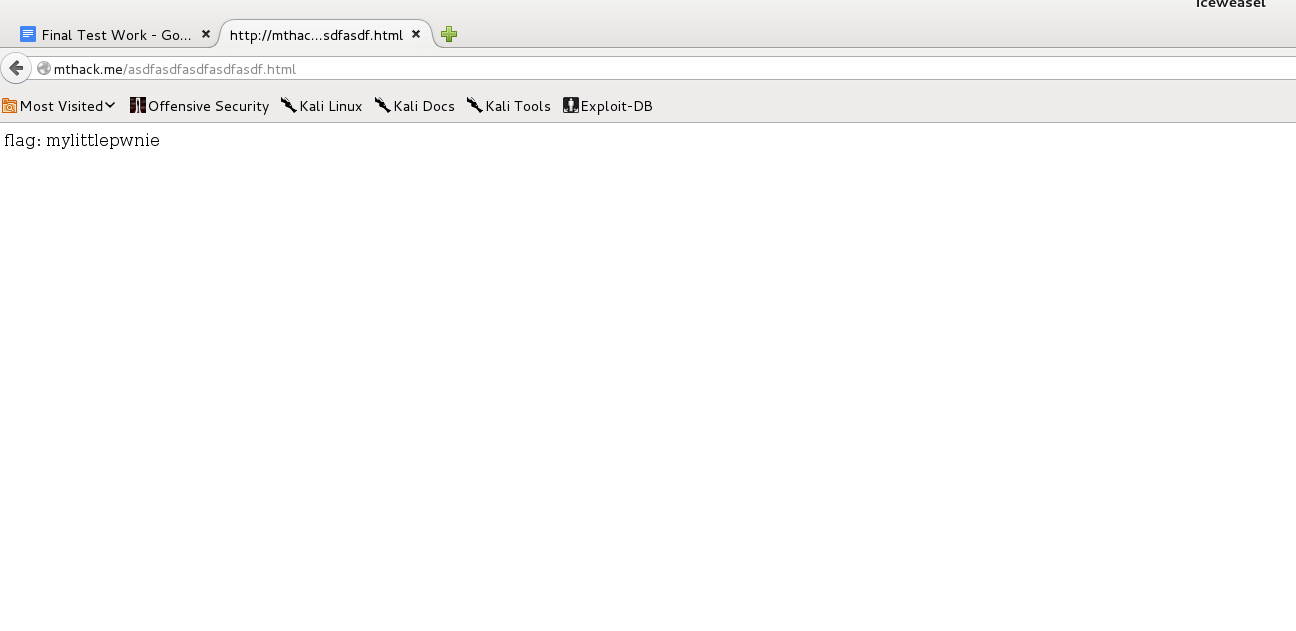
\includegraphics[scale=0.33]{mylittlepwnie.png}
\end{center}

\mychapter{7}{Summary}
The MHK domain has many vulnerabilities that I was able to exploit in order to find the flags dispersed throughout. My overall reccomendation is to never have Tomcat available to the public as it is a very vulnerable service, so that should be removed from mercury.mthack.me at all costs. It is also important to check the permissions on files in your file systems so that they can't be accessed through a web browser if the server has apache installed.\\
\newline
When compiling programs it is important to make sure that the compiler being used does not present the code in such an easy format for attackers to be able to exploit. File systems containing sensitive data should be encrypted to avoid it being stolen by an untrustworthy party. Lastly, WiFi traffic needs to be encrypted, preferably by WPA2. Finding the sensitive data in the pcap traffic was far too simple and could have been avoided if it was encrypted.
\clearpage

\bibliography{mybib}{}
\bibliographystyle{plain}

\end{document}